\chapter{Numerical Formulation}
\label{chapter:NF}
The previous chapter has shown the mathematical formulation for the single-phase flow equation, Eq. \ref{c3}. This chapter will show its discretization for solving it numerically. This discretization will be done by the finite-differences method, which according to \cite{Ertekin2001} is the method the most widely utilized by the industry. It consists of approximating the derivatives by finite differences, as illustrated in Figure \ref{fig:000};
\begin{figure}[H]
	\centering
	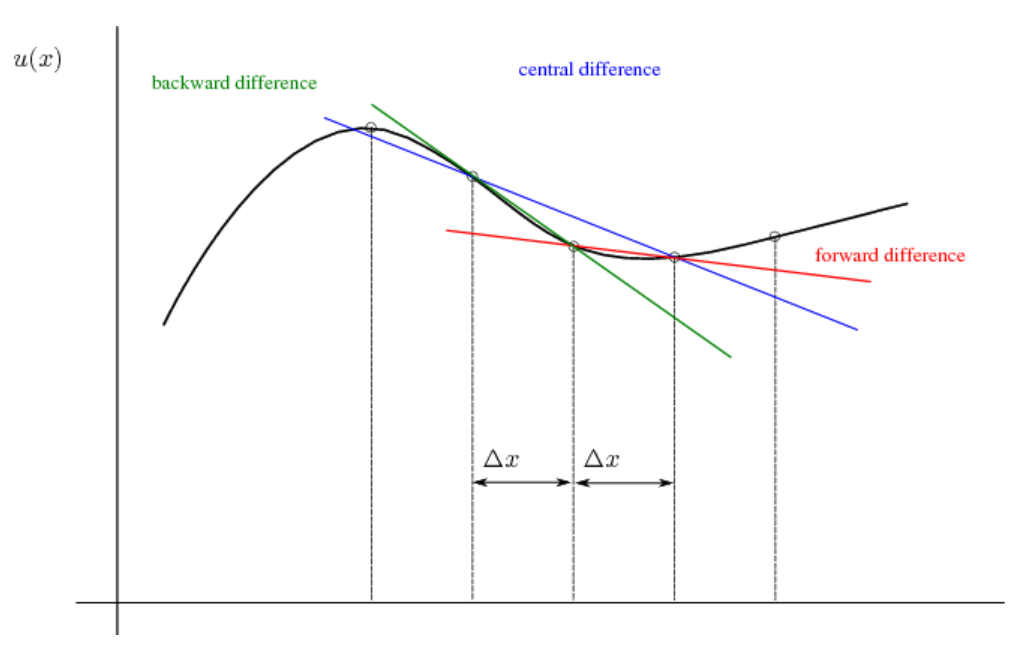
\includegraphics[width=1.0\textwidth]{000.png}\\
	\caption{Illustration of three finite differences methods: central difference, forward difference, and backward difference. Source: \cite{Heinzl1977}.}
	\label{fig:000}
\end{figure}
\noindent
For a given $f(x)$ function, its first-order derivative is defined as:
\begin{align}
\label{e0}
f'(x) = \lim_{\Delta x \to 0}\frac{f(x+\Delta x)-f(x)}{\Delta x}.
\end{align}
Assuming $\Delta x$ having a fixed, non-zero value, this limit can be approximated by:
\begin{align}
\label{e00}
f'(x) \approx \frac{f(x+\Delta x)-f(x)}{\Delta x}.
\end{align}
This is a finite-difference approach known as the forward difference method, since a posterior value, $x + \Delta x$, is utilized for the approximation. Another way of discretizing the Eq. \ref{e0} is:
\begin{align}
\label{e000}
f'(x) \approx \frac{f(x)-f(x - \Delta x)}{\Delta x},
\end{align}
this, on the other hand, is known as the backward difference method. In this approach, the previous value $x - \Delta x$ is utilized for calculating $f'(x)$. There is also the central difference method, in which both the $x - \Delta x$ and  $x + \Delta x$ are utilized for approximating the derivative:
\begin{align}
\label{e0000}
f'(x) \approx \frac{f(x + \Delta x)-f(x - \Delta x)}{2 \Delta x},
\end{align}
For the simulator developed in this project, the spatial derivatives will be approximated with the central difference and the time derivatives will be dealt with the backward difference. This approach is known as the BTCS method (backward-time, central-space) and characterizes an implicit model that, according to \cite{Ertekin2001}, is unconditionally stable.

\section{Grid Definition}
\label{chap:Grid Definition}
After doing a superimposition of a finite-block grid in a model of a petroleum reservoir, it is possible to approximate the continuum distribution of its proprieties (e.g. pressure, porosity, and permeability) by the average value of them inside each grid block. The grid-type utilized in the simulator will be the block-centered grid. \cite{Ertekin2001} shows the utilization of this type of grid for a unidimensional flow, as depicted in Figure \ref{f2}.
\begin{figure}[h]
	\centering
	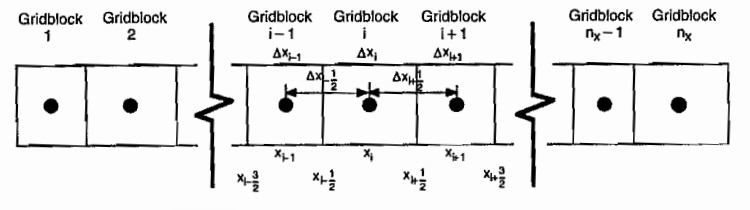
\includegraphics[width=1\textwidth]{f2.png}\\
	\caption{Unidimensional example of a block-centered grid. Source: \cite{Ertekin2001}.}
	\label{f2}
\end{figure}
For a simple illustration, a unidimensional reservor is represented by a  grid composed of $n_x$ blocks of predetermined dimensions, $\Delta x_i$, not necessarily equals, which must satisfy:
\nomenclature[R]{$n$}{Number of grid blocks in a given direction}
\nomenclature[U]{$x$}{$x$ direction}
\nomenclature[U]{$y$}{$y$ direction}
\nomenclature[U]{$z$}{$z$ direction}
\nomenclature[U]{$i$}{Index related to the $x$ direction}
\nomenclature[U]{$j$}{Index related to the $y$ direction}
\nomenclature[U]{$k$}{Index related to the $z$ direction}
\nomenclature[R]{$L$}{Total length of a reservoir}
	\begin{align}
	\label{e2.1}
	\sum_{i=1}^{n_x}\Delta x=L_x.
	\end{align}
In other words, the sum of the blocks' length should be equal to the reservoir length. Once the blocks are defined, the points in that the pressures are calculated are disposed of in their interior. In Cartesian coordinates, those points coincide with their center. The boundaries of a determined block with index $i$ are defined as $x_{i-\sfrac{1}{2}}$ and $x_{i+\sfrac{1}{2}}$, and their center is designated as $x_i$. Therefore, the following relations are valid for the block proprieties:
	\begin{align}
	\label{e2.2}
	x_i= (x_{i-\sfrac{1}{2}} + x_{i+\sfrac{1}{2}})
	\end{align}
	and
	\begin{align}
	\label{e2.3}
	x_i= x_{i+\sfrac{1}{2}} - x_{i-\sfrac{1}{2}}.
	\end{align}
Expanding this idea for a tridimensional, paralelepipedal reservoir, we can model it by dividing the grid into small volumetric elements that fits into the entire volume of the reservoir. For a grid block with indexes $i,j,k$, its center is defined in the point $(x_{i,j,k},y_{i,j,k},z_{i,j,k})$. Thus, the dimensions of this grid block would be $\Delta x_{i,j,k}$, $\Delta y_{i,j,k}$, $\Delta z_{i,j,k}$ and its volume $V_{i,j,k}$:
	\begin{align}
	\label{e00000}
	V_{i,j,k} = \Delta x_{i,j,k} \Delta y_{i,j,k} \Delta z_{i,j,k}.
	\end{align}
Threfore:
\nomenclature[R]{$V_{res}$}{Reservoir volume}
	\begin{align}
	\label{e000000}
	\sum_{i=1}^{n_x}\sum_{j=1}^{n_y}\sum_{k=1}^{n_z}\Delta x_{i,j,k} \Delta y_{i,j,k}\Delta z_{i,j,k}=V_{res}.
	\end{align}
Figure \ref{f0} illustrates such a model.
\begin{figure}[h]
	\centering
	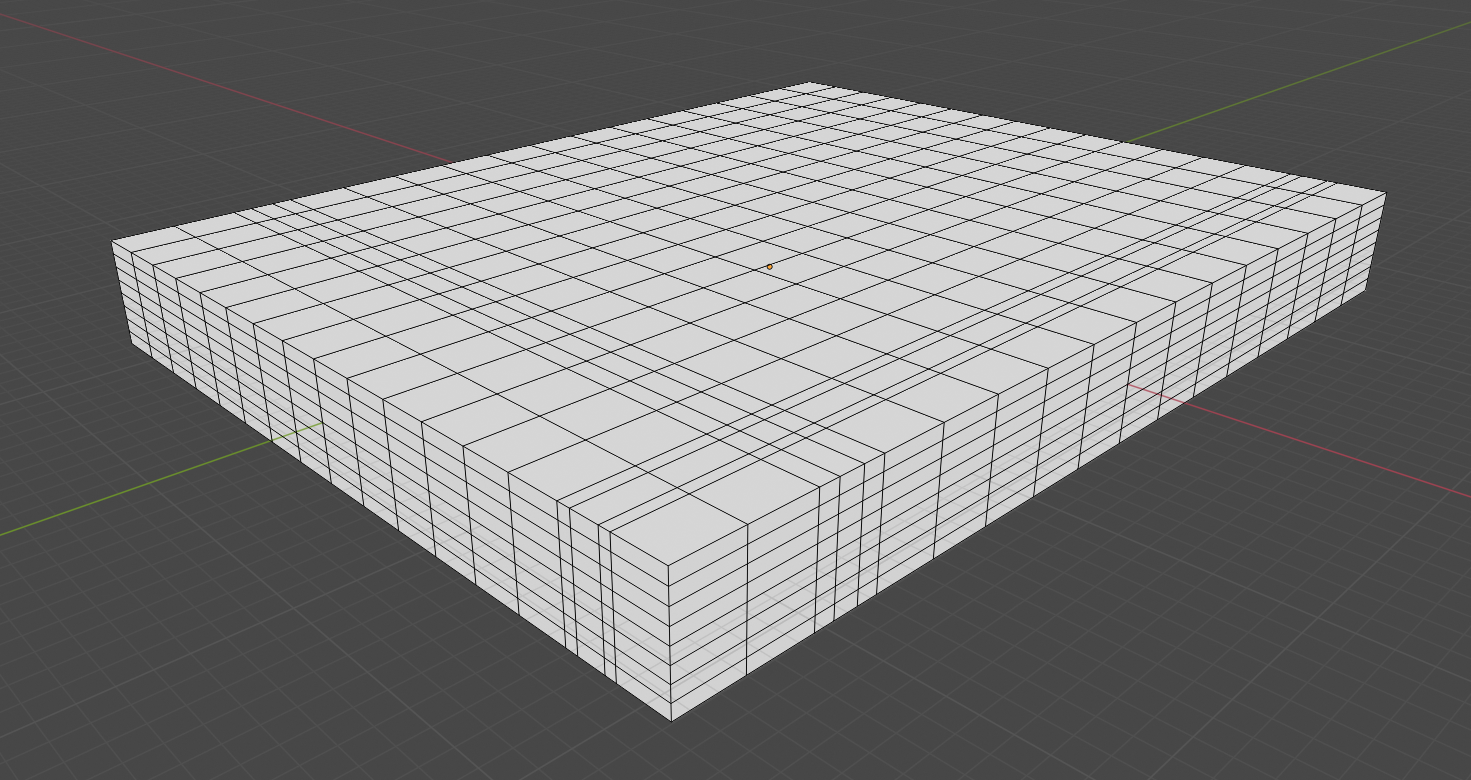
\includegraphics[width=1\textwidth]{00000.png}\\
	\caption{Example of a tridimensional grid representing a synthetic, parallelepipedal reservoir.}
	\label{f0}
\end{figure}
\noindent
As one can see, the grid blocks are allowed of having different sizes of $\Delta x$, $\Delta y$, and $\Delta z$ and they don't have to be equal from one grid block to another.

\section{Discretization in Space}
After the grid type has been defined, it is then possible to follow ahead with the discretization of the Eq. \ref{c3}.	 %According to \cite{Ertekin2001}, the approximations of spatial and temporal derivatives can be done with a Taylor series expansion of the dependent variable in the vicinity of grid points.
 Considering the term of the equation regarding the spatial derivative in the $x$ direction:
	\begin{align}
	\label{e2.4}
	\frac{\partial}{\partial x}\left( \beta_c \frac{A_x k_x}{\mu B}\frac{\partial p}{\partial x}\right) \Delta x
	\end{align}
Following the \cite{Ertekin2001} approach of approximating it by central differences, as shown in Eq. \ref{e0000}:
%Its central-differences approximations for a block with index $i$ is:
	\begin{multline}
	\label{e2.5}
	\frac{\partial}{\partial x}\left( \beta_c \frac{A_x k_x}{\mu B}\frac{\partial p}{\partial x}\right)_i \Delta x \\ \approx \frac{1}{\Delta x_i} \left[ \left( \beta_c \frac{A_x k_x}{\mu B}\frac{\partial p}{\partial x}\right)_{i+\sfrac{1}{2}} - \left( \beta_c \frac{A_x k_x}{\mu B}\frac{\partial p}{\partial x}\right)_{i-\sfrac{1}{2}}\right] \Delta x_i
	\end{multline}
That resulted not in an equation, but in an approximation. However, the approximation sign will be substituted for an equal sign in the following developments for the sake of simplicity. After performing this substitution and doing some rearrangements:
	\begin{multline}
	\label{e2.6}
	\frac{1}{\Delta x_i} \left[ \left( \beta_c \frac{A_x k_x}{\mu B}\frac{\partial p}{\partial x}\right)_{i+\sfrac{1}{2}} - \left( \beta_c \frac{A_x k_x}{\mu B}\frac{\partial p}{\partial x}\right)_{i-\sfrac{1}{2}}\right] \Delta x_i \\= \left( \beta_c \frac{A_x k_x}{\mu B}\right)_{i+\sfrac{1}{2}} \left(\frac{\partial p}{\partial x}\right)_{i+\sfrac{1}{2}} - \left( \beta_c \frac{A_x k_x}{\mu B}\right)_{i-\sfrac{1}{2}} \left(\frac{\partial p}{\partial x}\right)_{i-\sfrac{1}{2}}
	\end{multline}
For the derivative terms inside the brackets, their central-differences approximations are:
	\begin{align}
	\label{e2.7}
	\left(\frac{\partial p}{\partial x}\right)_{i+\sfrac{1}{2}}= \frac{p_{i+1}-p_i}{x_{i+1}-x_i}=\frac{p_{i+1}-p_i}{\Delta x_{1+\sfrac{1}{2}}}
	\end{align}
and:
	\begin{align}
	\label{e2.8}
	\left(\frac{\partial p}{\partial x}\right)_{i-\sfrac{1}{2}}= \frac{p_i-p_{i-1}}{x_{i+1}-x_i}=\frac{p_i-p_{i-1}}{\Delta x_{1+\sfrac{1}{2}}} .
	\end{align}
Substituting those into Eq. \ref{e2.6}:
	\begin{multline}
	\label{e2.9}
	\left( \beta_c \frac{A_x k_x}{\mu B}\right)_{i+\sfrac{1}{2}} \left(\frac{\partial p}{\partial x}\right)_{i+\sfrac{1}{2}} - \left( \beta_c \frac{A_x k_x}{\mu B}\right)_{i-\sfrac{1}{2}} \left(\frac{\partial p}{\partial x}\right)_{i-\sfrac{1}{2}}\\ = \left( \beta_c \frac{A_x k_x}{\mu B \Delta x}\right)_{i+\sfrac{1}{2}} (p_{i+1}-p_i) - \left( \beta_c \frac{A_x k_x}{\mu B \Delta x}\right)_{i-\sfrac{1}{2}} (p_i-p_{i-1})
	\end{multline}
This equation can be simplified even further by utilizing the definition of transmissibilities, as it is commonly done in the industry. The coefficients $T_{x_{i+\sfrac{1}{2}}}$ and $T_{x_{i-\sfrac{1}{2}}}$, known as the transmissibilities of the porous medium, are defined as:
\nomenclature[R]{$T_{i,j,k}$}{Transmissibility}
\nomenclature[R]{$G_{i,j,k}$}{Geometric transmissibility}
	\begin{align}
	\label{e2.10}
	T_{x_{i+\sfrac{1}{2}}}=\left( \beta_c \frac{A_x k_x}{\mu B \Delta x}\right)_{i+\sfrac{1}{2}}
	\end{align}
and
	\begin{align}
	\label{e2.11}
	T_{x_{i-\sfrac{1}{2}}}=\left( \beta_c \frac{A_x k_x}{\mu B \Delta x}\right)_{i-\sfrac{1}{2}}
	\end{align}
	\noindent
As indicated by their indexes, the transmissibilities are defined at the boundaries of the grid blocks, since they are utilized for evaluating the flow between adjacent blocks. Those transmissibilities have pressure-dependent factors, notably the FVF ($B$) and the viscosity ($\mu$); as well as pressure-independent ones: the transversal area ($A_x$), permeability ($k_x$), grid block length ($\Delta x$), and the transmissibility conversion factor ($\beta_c$). Splitting the transmissibility into a pressure-dependent and a pressure-independent factor simplifies the computational process, since the constant part can be calculated just one time for the entire simulation, and the pressure-dependent factor needs to be reevaluated in each iteration. Thus, rearranging the Eqs. \ref{e2.10} and \ref{e2.11}, the transmissibilities could be rewritten as:
\begin{align}
\label{e2.15}
T_{x_{i+\sfrac{1}{2}}}=\beta_c\left(\frac{A_x k_x}{\Delta x}\right)_{i+\sfrac{1}{2}} \left(\frac{1}{\mu B}\right)_{i+\sfrac{1}{2}}=\beta_c G_{x_{i+\sfrac{1}{2}}} \left(\frac{1}{\mu B}\right)_{i+\sfrac{1}{2}} ,
\end{align}
and
\begin{align}
\label{e2.16}
T_{x_{i-\sfrac{1}{2}}}=\beta_c\left(\frac{A_x k_x}{\Delta x}\right)_{i-\sfrac{1}{2}} \left(\frac{1}{\mu B}\right)_{i-\sfrac{1}{2}}=\beta_c G_{x_{i-\sfrac{1}{2}}} \left(\frac{1}{\mu B}\right)_{i-\sfrac{1}{2}} ,
\end{align}
where $G$ is the geometric transmissibility, representing the pressure-independent part. The pressure-dependent part can be calculated in function of the pressure at the faces of the blocks, by interpolating the FVF and viscosity with a value of pressure for a given fluid. The next subchapters will discuss in more detail the determination of those pressure-dependent variables. Substituting the Eqs. \ref{e2.10} and \ref{e2.11} into Eq. \ref{e2.9}:
	\begin{align}\nonumber
	\label{e2.13}
	&\left( \beta_c \frac{A_x k_x}{\mu B \Delta x}\right)_{i+\sfrac{1}{2}} (p_{i+1}-p_i) - \left( \beta_c \frac{A_x k_x}{\mu B \Delta x}\right)_{i-\sfrac{1}{2}} (p_i-p_{i-1})\\ &= T_{x_{i+\sfrac{1}{2}}} (p_{i+1}-p_i) - T_{x_{i-\sfrac{1}{2}}} (p_i-p_{i-1})
	\end{align}
Regarding the spatial derivative of the relative depth, its finite-difference approximation is:
	\begin{multline}
	\label{e2.5a}
	\frac{\partial}{\partial x}\left( \beta_c \frac{A_x k_x}{\mu B}\gamma\frac{\partial Z}{\partial x}\right)_i \Delta x \\ \approx \frac{\gamma}{\Delta x_i} \left[ \left( \beta_c \frac{A_x k_x}{\mu B}\frac{\partial Z}{\partial x}\right)_{i+\sfrac{1}{2}} - \left( \beta_c \frac{A_x k_x}{\mu B}\frac{\partial Z}{\partial x}\right)_{i-\sfrac{1}{2}}\right] \Delta x_i
	\end{multline}
It is possible to see that, except for the coefficient $\gamma$, the Eqs. \ref{e2.5} and \ref{e2.5a} are analogous. Taking a similar procedure for Eq. \ref{e2.5}:
	\begin{multline}
	\label{e2.13a}
	\frac{\gamma}{\Delta x_i} \left[ \left( \beta_c \frac{A_x k_x}{\mu B}\frac{\partial Z}{\partial x}\right)_{i+\sfrac{1}{2}} - \left( \beta_c \frac{A_x k_x}{\mu B}\frac{\partial Z}{\partial x}\right)_{i-\sfrac{1}{2}}\right] \Delta x_i \\ =  \gamma_{i+\sfrac{1}{2}} T_{x_{i+\sfrac{1}{2}}} (Z_{i+1}-Z_i) - \gamma_{i-\sfrac{1}{2}} T_{x_{i-\sfrac{1}{2}}} (Z_i-Z_{i-1})
	\end{multline}
Expanding the approximation of the spatial terms for the directions $y$ and $z$, and utilizing again the definition of transmissibility:
	\begin{multline}
\label{e2.5b}
\frac{\partial}{\partial y}\left( \beta_c \frac{A_y k_y}{\mu B}\gamma\frac{\partial Z}{\partial y}\right)_j \Delta y \\ =  \gamma_{j+\sfrac{1}{2}} T_{y_{j+\sfrac{1}{2}}} (Z_{j+1}-Z_j) - \gamma_{j-\sfrac{1}{2}} T_{y_{j-\sfrac{1}{2}}} (Z_j-Z_{j-1})
\end{multline}
and:
	\begin{multline}
\label{e2.5c}
\frac{\partial}{\partial z}\left( \beta_c \frac{A_z k_z}{\mu B}\gamma\frac{\partial Z}{\partial z}\right)_k \Delta z \\ =  \gamma_{k+\sfrac{1}{2}} T_{z_{k+\sfrac{1}{2}}} (Z_{k+1}-Z_k) - \gamma_{k-\sfrac{1}{2}} T_{z_{k-\sfrac{1}{2}}} (Z_k-Z_{k-1})
\end{multline}
After those approximations are applied in the single-phase flow equation, Eq. \ref{c3}, that partial-differential equation is then in the process of being substituted by a system of algebraic equations in the form:


 %and utilizing the definition of transmissibility, the Eq. \ref{c3} evaluated in a block with indexes $i,j,k$ can be rewritten as:
	\begin{align}\nonumber
	\label{e2.14}
	& T_{i+\sfrac{1}{2},j,k}(p_{i+1,j,k}-p_{i,j,k}) - T_{i-\sfrac{1}{2},j,k}(p_{i,j,k}-p_{i-1,j,k}) \nonumber +\\ &
	T_{i,j+\sfrac{1}{2},k}(p_{i,j+1,k}-p_{i,j,k}) - T_{i,j-\sfrac{1}{2},k}(p_{i,j,k}-p_{i,j-1,k}) \nonumber +\\ &
	T_{i,j,k+\sfrac{1}{2}}(p_{i,j,k+1}-p_{i,j,k}) - T_{i,j,k-\sfrac{1}{2}}(p_{i,j,k}-p_{i,j,k-1})
	 \nonumber +
	q_{sc_{i,j,k}} =\\ &
	\gamma_{i+\sfrac{1}{2},j,k} T_{i+\sfrac{1}{2},j,k}(Z_{i+1,j,k}-Z_{i,j,k}) - \gamma_{i-\sfrac{1}{2},j,k} T_{i-\sfrac{1}{2},j,k}(Z_{i,j,k}-Z_{i-1,j,k}) \nonumber +\\ &
	\gamma_{i,j+\sfrac{1}{2},k} T_{i,j+\sfrac{1}{2},k}(Z_{i,j+1,k}-Z_{i,j,k}) - \gamma_{i,j-\sfrac{1}{2},k} T_{i,j-\sfrac{1}{2},k}(Z_{i,j,k}-Z_{i,j-1,k}) \nonumber +\\ &
	\gamma_{i,j,k+\sfrac{1}{2}} T_{i,j,k+\sfrac{1}{2}}(Z_{i,j,k+1}-Z_{i,j,k}) - \gamma_{i,j,k-\sfrac{1}{2}} T_{i,j,k-\sfrac{1}{2}}(Z_{i,j,k}-Z_{i,j,k-1}) \nonumber +\\ &
	\frac {V_b}{\alpha_c}\frac{\partial}{\partial t}\left( \frac{\phi}{B}\right).
	\end{align}	
The indexes $i,j,k$ are utilized since this equation have to be calculated for each grid block of the model, then resulting in a system of $n_x n_y n_z$ equations, where $n_x$, $n_y$ and $n_z$ are the number of grid blocks in each direction for the model. However, Eq. \ref{e2.14} is still not complete since the time derivatives:
\begin{align}\nonumber
\frac {V_b}{\alpha_c}\frac{\partial}{\partial t}\left( \frac{\phi}{B}\right),
\end{align}
have not been discretized yet. The next subchapter will proceed with its discretization.

\section{Discretization in Time}

The previous subchapter has shown how the central-differences method has been utilized for approximating the spatial derivatives of the single-phase flow equation. On the other hand, the time derivatives will be approximated by backward difference. The approximation by backward difference of a derivative related to time $t^{n+1}$ is:
	\begin{align}
	\label{e2.17}
	\frac{\partial p}{\partial t} \approx \frac{p(t^{n+1})-p(t^n)}{\Delta t}.
	\end{align}
The following definitions will be utilized for the sake of simplicity:
	\begin{align}
	\label{e2.18}
	p^n=p(t^n)
	\end{align}
and
	\begin{align}
	\label{e2.19}
	p^{n+1}=p(t^{n+1}).
	\end{align}
Therefore, for a block with indexes $i,j,k$:
	\begin{align}
	\label{e2.20}
	\frac{\partial p_{i,j,k}}{\partial t} \approx \frac{p_{i,j,k}^{n+1}-p_{i,j,k}^n}{\Delta t}.
	\end{align}
Going back to the right term of the single-phase flow equation, Eq. \ref{c3}. Utilizing the chain rule of differentiation:
	\begin{align}
	\label{eqGamma4}
	\frac {V_b}{\alpha_c}\frac{\partial}{\partial t}\left( \frac{\phi}{B}\right) = \frac {V_b}{\alpha_c}\frac{\partial}{\partial p}\left( \frac{\phi}{B}\right)\frac{\partial p}{\partial t}.
	\end{align}
A new variable $\Gamma$ will be defined for facilitating the numerical calculations:
\nomenclature[G]{$\Gamma_{i,j,k}$}{Accumulation coefficient}
	\begin{align}
	\label{eqGamma5}
	\Gamma = \frac {V_b}{\alpha_c}\frac{\partial}{\partial p}\left( \frac{\phi}{B}\right).
	\end{align}
 Expanding the derivatives of $\phi / B$ in relation to the pressure and considering a constant $c_f$ for the changes of pressure: % TODO: Develop this equation if have time
	\begin{align}
	\label{eqGamma3}
	\Gamma^{n,n+1}_{i,j,k} = \frac {V_{b_{i,j,k}}}{\alpha_c} \left[ \frac{\phi^{n+1}_{i,j,k} c_f}{B^{n+1}_{i,j,k}} + \frac{\phi^n_{i,j,k}}{B^n_{i,j,k}} \frac{ \left( B^n_{i,j,k}/B^{n+1}_{i,j,k}-1\right) } { (p^{n+1}_{i,j,k} - p^{n}_{i,j,k}) } \right].
	\end{align}
The index $n,n+1$ in $\Gamma$ means that some parameters in the $\Gamma$ definition are evaluated at $n$ and others at $n+1$. Utilizing the concept of the backward-difference method shown in Eq. \ref{e000}. 
	\begin{multline}
	\label{eqGamma2}
	\frac {V_{b_{i,j,k}}}{\alpha_c} \left[ \frac{\phi^{n+1}_{i,j,k} c_f}{B^{n+1}_{i,j,k}} + \frac{\phi^n_{i,j,k}}{B^n_{i,j,k}} \frac{ \left( B^n_{i,j,k}/B^{n+1}_{i,j,k}-1\right) } { (p^{n+1}_{i,j,k} - p^{n}_{i,j,k}) } \right] \frac{\partial p}{\partial t} = \Gamma^{n,n+1}_{i,j,k} \frac{(p^{n+1}_{i,j,k} - p^{n}_{i,j,k})}{\Delta t}.
	\end{multline}
This is the discretized form of the time-dependent term of the single-phase flow equation. Applying this definition back in Eq. \ref{e2.14}:
	\begin{align}\nonumber
	\label{e2.21}
	& T^{n+1}_{i+\sfrac{1}{2},j,k}(p^{n+1}_{i+1,j,k}-p^{n+1}_{i,j,k}) - T^{n+1}_{i-\sfrac{1}{2},j,k}(p^{n+1}_{i,j,k}-p^{n+1}_{i-1,j,k}) \nonumber +\\ &
	T^{n+1}_{i,j+\sfrac{1}{2},k}(p^{n+1}_{i,j+1,k}-p^{n+1}_{i,j,k}) - T^{n+1}_{i,j-\sfrac{1}{2},k}(p^{n+1}_{i,j,k}-p^{n+1}_{i,j-1,k}) \nonumber +\\ &
	T^{n+1}_{i,j,k+\sfrac{1}{2}}(p^{n+1}_{i,j,k+1}-p^{n+1}_{i,j,k}) - T^{n+1}_{i,j,k-\sfrac{1}{2}}(p^{n+1}_{i,j,k}-p^{n+1}_{i,j,k-1})
	\nonumber +
	q^{n+1}_{sc_{i,j,k}} =\\ &
	\gamma^{n+1}_{i+\sfrac{1}{2},j,k} T^{n+1}_{i+\sfrac{1}{2},j,k}(z^{n+1}_{r_{i+1,j,k}}-z^{n+1}_{r_{i,j,k}}) - \gamma^{n+1}_{i-\sfrac{1}{2},j,k} T^{n+1}_{i-\sfrac{1}{2},j,k}(z^{n+1}_{r_{i,j,k}}-z^{n+1}_{r_{i-1,j,k}}) \nonumber +\\ &
	\gamma^{n+1}_{i,j+\sfrac{1}{2},k} T^{n+1}_{i,j+\sfrac{1}{2},k}(z^{n+1}_{r_{i,j+1,k}}-z^{n+1}_{r_{i,j,k}}) - \gamma^{n+1}_{i,j-\sfrac{1}{2},k} T^{n+1}_{i,j-\sfrac{1}{2},k}(z^{n+1}_{r_{i,j,k}}-z^{n+1}_{r_{i,j-1,k}}) \nonumber +\\ &
	\gamma^{n+1}_{i,j,k+\sfrac{1}{2}} T^{n+1}_{i,j,k+\sfrac{1}{2}}(z^{n+1}_{r_{i,j,k+1}}-z^{n+1}_{r_{i,j,k}}) - \gamma^{n+1}_{i,j,k-\sfrac{1}{2}} T^{n+1}_{i,j,k-\sfrac{1}{2}}(z^{n+1}_{r_{i,j,k}}-z^{n+1}_{r_{i,j,k-1}}) \nonumber +\\ &
	\frac{\Gamma_{i,j,k}^{n,n+1}}{\Delta t} (p_{i,j,k}^{n+1}-p_{i,j,k}^n).
	\end{align}
Finally, this is the single-phase flow equation discretized by the BTCS method. It is necessary to set boundary conditions for the solution of this equation. The problem considers a sealed reservoir, which means a reservoir with a flow rate equals to zero in the boundaries. That can be modeled by setting the transmissibilities equal to zero for the faces of the grid blocks that are in a boundary of the reservoir. The next section will show another form of representing \ref{e2.21} for its simplification.	

\section{Matrix Notation}

\cite{Ertekin2001} defines a matrix coefficients notation that simplifies the utilization of the Eq.\ref{e2.21}. Rearranging the equation:
\begin{align}\nonumber
\label{rearranjo}
& T^{n+1}_{i,j,k+\sfrac{1}{2}} p^{n+1}_{i,j,k+1} + T^{n+1}_{i,j+\sfrac{1}{2},k} p^{n+1}_{i,j+1,k} + T^{n+1}_{i+\sfrac{1}{2},j,k} p^{n+1}_{i+1,j,k} \nonumber -\\ &
\Big( \frac{\Gamma_{i,j,k}^{n+1}}{\Delta t} + T^{n+1}_{i,j,k+\sfrac{1}{2}} + T^{n+1}_{i,j+\sfrac{1}{2},k} + T^{n+1}_{i+\sfrac{1}{2},j,k} \nonumber +\\ &
T^{n+1}_{i,j,k-\sfrac{1}{2}} + T^{n+1}_{i,j-\sfrac{1}{2},k} + T^{n+1}_{i-\sfrac{1}{2},j,k} \Big) p^{n+1}_{i,j,k} \nonumber +\\ &
T^{n+1}_{i,j,k-\sfrac{1}{2}} p^{n+1}_{i,j,k-1} + T^{n+1}_{i,j-\sfrac{1}{2},k} p^{n+1}_{i,j-1,k} + T^{n+1}_{i-\sfrac{1}{2},j,k} p^{n+1}_{i-1,j,k} 	\nonumber =\\ &
\gamma^{n+1}_{i+\sfrac{1}{2},j,k} T^{n+1}_{i+\sfrac{1}{2},j,k}(z^{n+1}_{r_{i+1,j,k}}-z^{n+1}_{r_{i,j,k}}) - \gamma^{n+1}_{i-\sfrac{1}{2},j,k} T^{n+1}_{i-\sfrac{1}{2},j,k}(z^{n+1}_{r_{i,j,k}}-z^{n+1}_{r_{i-1,j,k}}) \nonumber +\\ &
\gamma^{n+1}_{i,j+\sfrac{1}{2},k} T^{n+1}_{i,j+\sfrac{1}{2},k}(z^{n+1}_{r_{i,j+1,k}}-z^{n+1}_{r_{i,j,k}}) - \gamma^{n+1}_{i,j-\sfrac{1}{2},k} T^{n+1}_{i,j-\sfrac{1}{2},k}(z^{n+1}_{r_{i,j,k}}-z^{n+1}_{r_{i,j-1,k}}) \nonumber +\\ &
\gamma^{n+1}_{i,j,k+\sfrac{1}{2}} T^{n+1}_{i,j,k+\sfrac{1}{2}}(z^{n+1}_{r_{i,j,k+1}}-z^{n+1}_{r_{i,j,k}}) - \gamma^{n+1}_{i,j,k-\sfrac{1}{2}} T^{n+1}_{i,j,k-\sfrac{1}{2}}(z^{n+1}_{r_{i,j,k}}-z^{n+1}_{r_{i,j,k-1}})\nonumber -\\ &
\frac{\Gamma_{i,j,k}^{n,n+1}}{\Delta t} p_{i,j,k}^n - q^{n+1}_{sc_{i,j,k}}
\end{align}
By looking at this equation, one can see that the transmissibilities are evaluated in different faces of a grid block of indexes $i,j,k$. The idea of the matrix coefficient notation is to assign the transmissibilities evaluated in each face with a letter that symbolizes the face. Figure \ref{fig:3} shows the definition of some of those new coefficients.
 \begin{figure}[h]
 	\centering
 	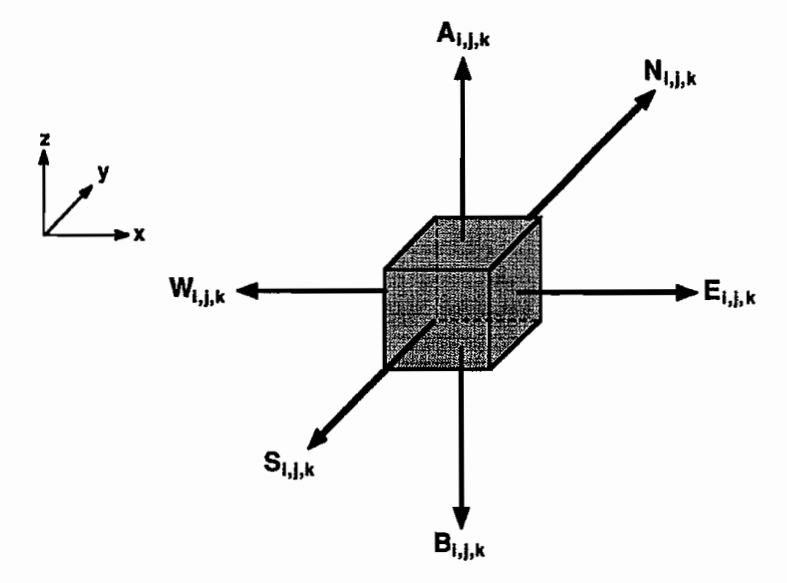
\includegraphics[width=0.65\textwidth]{3.png}\\
 	\caption{Illustration of the matrix coefficients utilized for representing the transmissibilities. Source: \cite{Ertekin2001}.}
 	\label{fig:3}
 \end{figure}
The following set of equations show the definition of those new coefficients:
	\begin{gather}\label{coef1}
	W_{i,j,k}^{n+1}=T_{i-\sfrac{1}{2},j,k}^{n+1},\\
	E_{i,j,k}^{n+1}=T_{i+\sfrac{1}{2},j,k}^{n+1},\\
	S_{i,j,k}^{n+1}=T_{i,j-\sfrac{1}{2},k}^{n+1},\\
	N_{i,j,k}^{n+1}=T_{i,j+\sfrac{1}{2},k}^{n+1},\\
	B_{i,j,k}^{n+1}=T_{i,j,k+\sfrac{1}{2}}^{n+1},\\
	A_{i,j,k}^{n+1}=T_{i,j,k-\sfrac{1}{2}}^{n+1},\\
	C_{i,j,k}^{n+1}=-\left(\frac{\Gamma_{i,j,k}^{n,n+1}}{\Delta t} + W_{i,j,k}^{n+1}+E_{i,j,k}^{n+1}+S_{i,j,k}^{n+1}+N_{i,j,k}^{n+1}+B_{i,j,k}^{n+1}+A_{i,j,k}^{n+1}\right),\\
	W_{G_{i,j,k}}^{n+1}=\gamma_{i-\sfrac{1}{2},j,k}^{n+1}T_{i-\sfrac{1}{2},j,k}^{n+1},\\
	E_{G_{i,j,k}}^{n+1}=\gamma_{i+\sfrac{1}{2},j,k}^{n+1}T_{i+\sfrac{1}{2},j,k}^{n+1},\\
	S_{G_{i,j,k}}^{n+1}=\gamma_{i,j-\sfrac{1}{2},k}^{n+1}T_{i,j-\sfrac{1}{2},k}^{n+1},\\
	N_{G_{i,j,k}}^{n+1}=\gamma_{i,j+\sfrac{1}{2},k}^{n+1}T_{i,j+\sfrac{1}{2},k}^{n+1},\\
	B_{G_{i,j,k}}^{n+1}=\gamma_{i,j,k+\sfrac{1}{2}}^{n+1}T_{i,j,k-\sfrac{1}{2}}^{n+1},\\
	A_{G_{i,j,k}}^{n+1}=\gamma_{i,j,k-\sfrac{1}{2}}^{n+1}T_{i,j,k+\sfrac{1}{2}}^{n+1},\\
	C_{G_{i,j,k}}^{n+1}=-\left( W_{G_{i,j,k}}^{n+1}+E_{G_{i,j,k}}^{n+1}+S_{G_{i,j,k}}^{n+1}+N_{G_{i,j,k}}^{n+1}+B_{G_{i,j,k}}^{n+1}+A_{G_{i,j,k}}^{n+1}\right)
	\end{gather}
\nomenclature[R]{$E_{i,j,k}$}{Transmissibility coefficient of $p_{i+\sfrac{1}{2},j,k}$ in matrix notation}
\nomenclature[R]{$W_{i,j,k}$}{Transmissibility coefficient of $p_{i-\sfrac{1}{2},j,k}$ in matrix notation}
\nomenclature[R]{$N_{i,j,k}$}{Transmissibility coefficient of $p_{i,j+\sfrac{1}{2},k}$ in matrix notation}
\nomenclature[R]{$S_{i,j,k}$}{Transmissibility coefficient of $p_{i,j-\sfrac{1}{2},k}$ in matrix notation}
\nomenclature[R]{$A_{i,j,k}$}{Transmissibility coefficient of $p_{i,j,k+\sfrac{1}{2}}$ in matrix notation}
\nomenclature[R]{$B_{i,j,k}$}{Transmissibility coefficient of $p_{i,j,k-\sfrac{1}{2}}$ in matrix notation}
\nomenclature[R]{$C_{i,j,k}$}{Transmissibility coefficient of $p_{i,j,k}$ in matrix notation}
\nomenclature[R]{$E_{G_{i,j,k}}$}{Modified transmissibility coefficient for $Z_{i+\sfrac{1}{2},j,k}$ in matrix notation}
\nomenclature[R]{$W_{G_{i,j,k}}$}{Modified transmissibility coefficient for $Z_{i-\sfrac{1}{2},j,k}$ in matrix notation}
\nomenclature[R]{$N_{G_{i,j,k}}$}{Modified transmissibility coefficient for $Z_{i,j+\sfrac{1}{2},k}$ in matrix notation}
\nomenclature[R]{$S_{G_{i,j,k}}$}{Modified transmissibility coefficient for $Z_{i,j-\sfrac{1}{2},k}$ in matrix notation}
\nomenclature[R]{$A_{G_{i,j,k}}$}{Modified transmissibility coefficient for $Z_{i,j,k+\sfrac{1}{2}}$ in matrix notation}
\nomenclature[R]{$B_{G_{i,j,k}}$}{Modified transmissibility coefficient for $Z_{i,j,k-\sfrac{1}{2}}$ in matrix notation}
\nomenclature[R]{$C_{G_{i,j,k}}$}{Modified transmissibility coefficient for $Z_{i,j,k}$ in matrix notation}
and
\nomenclature[R]{$Q_{i,j,k}$}{Known right side of the single-phase flow equation in matrix notation, volume at standard conditions}
%BRENO:O Q avalia a pressão no passo de tempo "n" e os demais parâmetros no passo de tempo "n+1", portanto escolhi deixa-lo com superindice "n, n+1"
	\begin{multline}\label{coef2}
	Q_{i,j,k}^{n,n+1}=-\Big(\frac{\Gamma_{i,j,k}^{n,n+1}}{\Delta t}p_{i,j,k}^n+ q_{sc_{i,j,k}} - W_{G_{i,j,k}}^{n+1}Z_{i-\sfrac{1}{2},j,k}^{n+1}-E_{G_{i,j,k}}^{n+1}Z_{i+\sfrac{1}{2},j,k}^{n+1}\\-S_{G_{i,j,k}}^{n+1}Z_{i,j-\sfrac{1}{2},k}^{n+1}-N_{G_{i,j,k}}^{n+1}Z_{i,j+\sfrac{1}{2},k}^{n+1}-B_{G_{i,j,k}}^{n+1}Z_{i,j,k-\sfrac{1}{2}}^{n+1}-A_{G_{i,j,k}}^{n+1}Z_{i,j,k+\sfrac{1}{2}}^{n+1}\Big).
	\end{multline}
Applying those new definitions in the \ref{e2.21}:
	\begin{multline}
	\label{matrix}
	W^{n+1}_{i,j,k}p^{n+1}_{i-1,j,k}+E^{n+1}_{i,j,k}p^{n+1}_{i+1,j,k}+S^{n+1}_{i,j,k}p^{n+1}_{i,j-1,k}\\+N^{n+1}_{i,j,k}p^{n+1}_{i,j+1,k}+B^{n+1}_{i,j,k}p^{n+1}_{i,j,k-1}+A^{n+1}_{i,j,k}p^{n+1}_{i,j,k+1}+C^{n+1}_{i,j,k}p^{n+1}_{i,j,k}=Q^{n, n+1}_{i,j,k}.
	\end{multline}
This is the single-phase flow equation discretized with the BTCS method and simplified with the \cite{Ertekin2001} matrix coefficients notation. For calculating the pressure at the next time step, $p^{n + 1}$, the simulator has to compute this equation for every grid block, for the entire model. Thus, this will generate a system of $n$ equations, in which $n$ is the total number of the blocks in the grid. However, this system of equations is non-linear because the coefficients $W$, $E$, $S$, $N$, $A$, $B$, $C$, $Q$ have terms that depend on the pressure. The next subchapter will show how this problem will be handled by transforming this non-linear system of equations into a linear one.

\section{Linearization}
\label{linearization}
As discussed in the previous subchapter, the non-linear system of equations represented by Eq. \ref{e2.21} needs to be linearized for enabling it to be solved by methods of linear algebra. There are several different ways for doing that but this project approaches it by what \cite{Ertekin2001} describes as the simple iteration of the transmissibility terms. There are more efficient techniques of linearization for achieving a faster convergency, like the Newton-Raphson method, but their implementation is more complex and doesn't fit in the initial scope of this project. In terms of accuracy, there is no significant difference between those methods, as shown in the results when compared to industry-standard software.
	\begin{figure}[H]
	\centering
	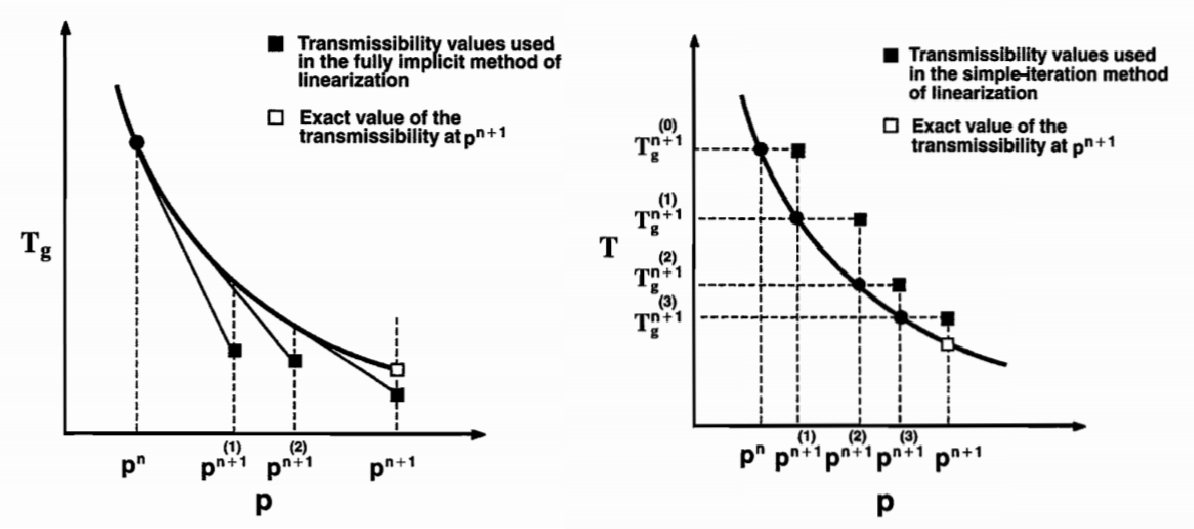
\includegraphics[width=1.0\textwidth]{0000000.png}\\
	\caption{The convergence of the Newton-Raphson method in comparison with the Simple Iteration of the Transmissibility Terms. Source: \cite{Ertekin2001}.}
	\label{fig:0000}
	\end{figure}
The problem described at the end of the previous subchapter is that the pressure coefficients in Eq. \ref{e2.21} are also pressure-dependent variables, thus the resultant system of equation is non-linear. The simple iteration described by \cite{Ertekin2001} consists of evaluating those dependent variables utilizing the pressure value of one iteration level bellow the pressure level utilized for solving the linear system. By the definition of transmissibility from the Eqs. \ref{e2.15} and \ref{e2.16}, using $\nu$ is the iteration index:
	\begin{align}
	\label{e2.22}
	T^{n+1}_{i\pm \sfrac{1}{2},j,k} \approx T^{\stackrel{(\nu)}{n+1}}_{i\pm \sfrac{1}{2},j,k}= \beta_c\left(\frac{A_x k_x}{\Delta x}\right)_{i\pm \sfrac{1}{2},j,k}\left( \frac{1}{\mu B}\right)_{i\pm \sfrac{1}{2},j,k}^{\stackrel{(\nu)}{n+1}}.
	\end{align}
Using the concept of geometric factor, $G_{i,j,k}$, defined in Eq. \ref{e2.16}:
	\begin{align}
	\label{e2.23}
	T^{\stackrel{(\nu)}{n+1}}_{i\pm \sfrac{1}{2},j,k}= \beta_c G_{i\pm \sfrac{1}{2},j,k}\left( \frac{1}{\mu B}\right)_{i\pm 	\sfrac{1}{2},j,k}^{\stackrel{(\nu)}{n+1}}.
	\end{align}
The variables inside the transmissibility factor are evaluated in the faces of the grid blocks, while the grid block proprieties are assigned in the center of the blocks for a block-centered grid. Therefore, it is necessary to determine the proprieties at the faces of the blocks by applying some kind of average. The method utilized in this project has been the harmonic averaging, $A_{-1}$, which is recomended by \cite{Ertekin2001} and defined as:
\nomenclature[R]{$A_{-1}$}{Harmonic average operator}
\nomenclature[R]{a}{Generic number for the harmonic average equation}
\nomenclature[R]{n}{Number of elements for being averaged}
\begin{align}
\label{geofactor1}
\frac{1}{A_{-1}(a)}=\frac{1}{n}\left(\frac{1}{a_1}+\frac{1}{a_2}+...+\frac{1}{a_n}\right),
\end{align}
where $n$ is the number of the averaged propriety $a$. Thus, the geometric transmissibility at the face $i+\sfrac{1}{2},j,k$ can be calculated by:
\begin{align}
\label{geofactor2}
\frac{1}{G_{i+\sfrac{1}{2},j,k}} = \frac{1}{A_{-1}(G_{i,j,k},G_{i+ 1,j,k})}=\frac{1}{2}\left[\left(\frac{\Delta x}{A_x k_x}\right)_{i,j,k}+\left(\frac{\Delta x}{A_x k_x}\right)_{i + 1,j,k}\right],
\end{align}
\begin{multline}
\label{geofactor3}
\frac{1}{A_{-1}(G_{i,j,k},G_{i+ 1,j,k})}=\\\frac{1}{2}\left[\frac{
\Delta x_{i + 1,j,k}(A_{x_{i,j,k}}k_{x_{i,j,k}})+\Delta x_{i,j,k}(A_{x_{i + 1,j,k}}k_{x_{i + 1,j,k}})}{A_{x_{i,j,k}}A_{x_{i + 1,j,k}}K_{x_{i,j,k}}K_{x_{i + 1,j,k}}}\right],
\end{multline}
\begin{multline}
\label{geofactor4}
G_{i+ \sfrac{1}{2},j,k}=A_{-1}(G_{i,j,k},G_{i+ 1,j,k})=\\\frac{2 A_{x_{i,j,k}}A_{x_{i + 1,j,k}}K_{x_{i,j,k}}K_{x_{i + 1,j,k}}}{
	\Delta x_{i + 1,j,k}(A_{x_{i,j,k}}k_{x_{i,j,k}})+\Delta x_{i,j,k}(A_{x_{i + 1,j,k}}k_{x_{i + 1,j,k}})}.
\end{multline}
The same approach can be utilized for calculating the geometric transmissibilities at the different faces of the grid blocks. 

The software developed in this project requires a fluid table as a parameter for the simulation. This table should relate the pressure-dependent proprieties (FVF, viscosity and specific weight) to a set of pressure values. In order to obtain those proprieties for a given face of the grid block, an interpolation is done for the value of pressure at that grid-block's face. Figures \ref{fig:0fluid_table1} to \ref{fig:0fluid_table3} show an example of relationships between pressure and those pressure-dependent proprieties, as well as a linear regression utilized for interpolating their values for a given pressure.
\begin{figure}[H]
	\centering
	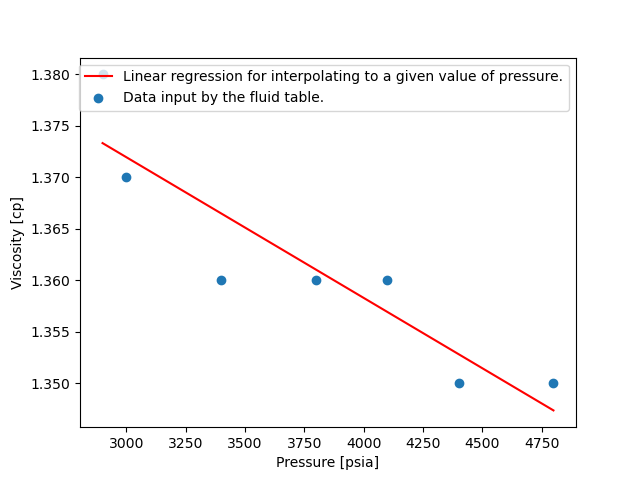
\includegraphics[width=0.7\textwidth]{0fluid_table1.png}\\
	\caption{Example of a relationship between pressure and viscosity, as well as a linear regression utilizing for interpolating the viscosity for a given value of pressure.}
	\label{fig:0fluid_table1}
\end{figure}
Thus, the pressure-dependent factor of the transmissibility can be written as:
\begin{align}
\label{e2.24}
\left(\frac{1}{\mu B}\right)_{i\pm\sfrac{1}{2},j,k}^{\stackrel{(\nu)}{n+1}}=\left(\frac{1}{\mu_{i\pm\sfrac{1}{2},j,k} B_{i\pm\sfrac{1}{2},j,k}}\right)^{\stackrel{(\nu)}{n+1}}.
\end{align}
The pressure at the grid-block's faces will be determined by an arithmetic mean of the pressures at the center of the grid blocks:
\begin{align}
\label{e2.25}
p_{i\pm\sfrac{1}{2},j,k}^{\stackrel{(\nu)}{n+1}}=\frac{p^{\stackrel{(\nu)}{n+1}}_{i\pm\sfrac{1}{2},j,k}+p^{\stackrel{(\nu)}{n+1}}_{i,j,k}}{2}.
\end{align}
\begin{figure}[H]
	\centering
	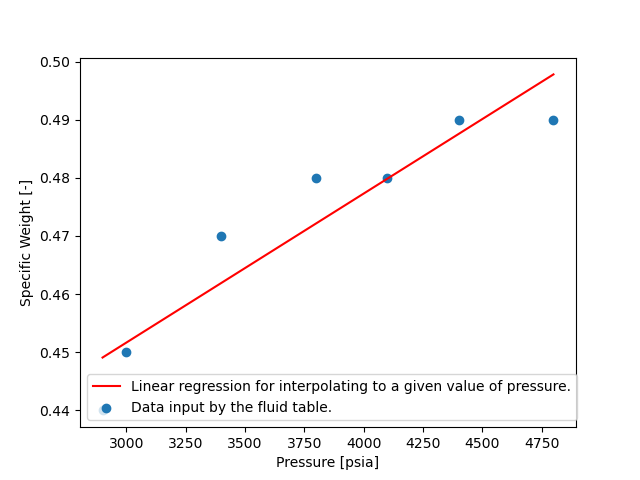
\includegraphics[width=0.7\textwidth]{0fluid_table2.png}\\
	\caption{Example of a relationship between pressure and specific weight, as well as a linear regression utilizing for interpolating the specific weight for a given value of pressure.}
	\label{fig:0fluid_table2}
\end{figure}
\begin{figure}[H]
	\centering
	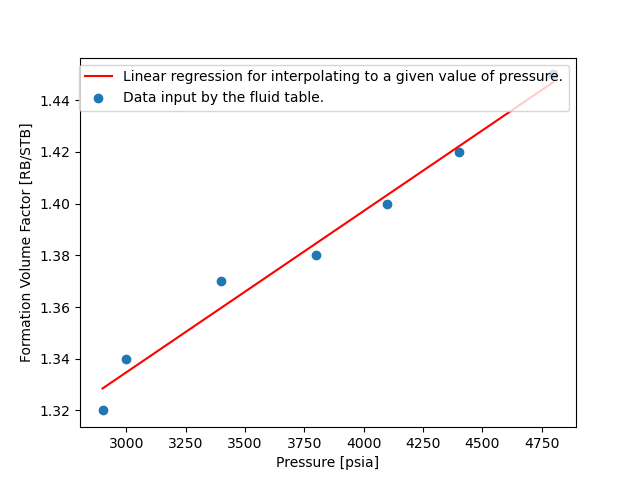
\includegraphics[width=0.7\textwidth]{0fluid_table3.png}\\
	\caption{Example of a relationship between pressure and FVF, as well as a linear regression utilizing for interpolating the FVF for a given value of pressure.}
	\label{fig:0fluid_table3}
\end{figure}
\noindent
After calculating those proprieties, it is then possible to obtain the transmissibilities in the iteration level $\nu$. Applying the iteration indexes in the Eq. \ref{matrix}:
	\begin{multline}
	\label{matrix2}
	W^{\stackrel{(\nu)}{n+1}}_{i,j,k}p^{\stackrel{\Large{(\nu+1)}}{n+1}}_{i-1,j,k}+E^{\stackrel{(\nu)}{n+1}}_{i,j,k}p^{\stackrel{(\nu+1)}{n+1}}_{i+1,j,k}+S^{\stackrel{(\nu)}{n+1}}_{i,j,k}p^{\stackrel{(\nu+1)}{n+1}}_{i,j-1,k}\\+N^{\stackrel{(\nu)}{n+1}}_{i,j,k}p^{\stackrel{(\nu+1)}{n+1}}_{i,j+1,k}+B^{\stackrel{(\nu)}{n+1}}_{i,j,k}p^{\stackrel{(\nu+1)}{n+1}}_{i,j,k-1}+A^{\stackrel{(\nu)}{n+1}}_{i,j,k}p^{\stackrel{(\nu+1)}{n+1}}_{i,j,k+1}+C^{\stackrel{(\nu)}{n+1}}_{i,j,k}p^{\stackrel{(\nu+1)}{n+1}}_{i,j,k}=Q^{\stackrel{(\nu)}{n,n+1}}_{i,j,k}.
	\end{multline}
This is the main equation utilized in the simulation: the single-phase flow equation discretized by the BTCS method and linearized by the simple iteration of the transmissibility terms. This equation should be calculated for each grid block at each iteration. That would result in a linear system of equations for being solved at each iteration. The next chapter will show how the well will be modeled for being implemented in this equation prior to its solution.

